\documentclass[11pt]{book}

\usepackage[width=7.0in, height=9.0in, top=1.0in, papersize={8.5in,11in}]{geometry}
\usepackage[pdftex]{graphicx}
%\usepackage{datetime}
\usepackage{anyfontsize}
\usepackage{hyperref}
\usepackage{t1enc}
\usepackage{wrapfig}
\usepackage{verbatim}
\usepackage{algorithm}
\usepackage{algorithmic}
\usepackage{framed}
\usepackage{pdfpages}
\usepackage{listings}
\lstset{language=C}

\lstset{language=python,frame=ltrb,framesep=5pt,basicstyle=\normalsize,
 keywordstyle=\ttfamily\color{DarkRed},
%morecomment=[n][\textbf]{In\ [}{]\:},
%morecomment=[n][\textbf]{Out\ [}{]\:},
morecomment=[s][\color{blue}]{In\ [}{]\:},
morecomment=[s][\color{red}]{Out[}{]\:},
identifierstyle=\ttfamily\color{DarkBlue}\bfseries,
commentstyle=\color{DarkGreen},
stringstyle=\ttfamily,
showstringspaces=false,tabsize = 3}


\lstdefinelanguage{shell} {
commentstyle = \color{black},
keywordstyle = \color{black},
stringstyle = \color{black},
identifierstyle = \color{black},
morecomment=[s][\color{blue}]{In\ [}{]\:},
morecomment=[s][\color{red}]{Out[}{]\:},
 }

\pagestyle{empty}

\usepackage{helvet}
\renewcommand{\familydefault}{\sfdefault}

\begin{document}

\noindent{\fontsize{16}{16}\selectfont Sprint Report \#5}
\\[3mm]
% !TEX root = sprints.tex
\noindent \Large{\textbf{Summary}}\\
\normalsize Team Expeditus was unfortunately unable to complete the tasks for sprint 5, but the team was able to make measurable progress towards the goals. After deciding not to pursue simulation, the team members began to focus on message passing and offboard control between the flight controller and the Odroid. After multiple issues with multiple approaches to the AR tag tracking, the team was able to successfully get the AR Track Alvar library up and running.
\vspace{5mm}
\\
\noindent \Large{\textbf{Team Work}}
\normalsize
\begin{itemize}
\item \textbf{Jonathan Dixon:} Worked AR tracking.
\item \textbf{Dylan Geyer:} Worked on AR tracking.
\item \textbf{Christopher Smith:} Worked on message passing and offboard control. 
\item \textbf{Steven Huerta:} Worked on AR tracking. 
\end{itemize}

\vspace{5mm}
\noindent\Large{\textbf{Uncompleted Tasks}}\\
\vspace{2mm}\\
\noindent \large{\textbf{As an owner, I want the UAV to autonomously land on the landing pad without damaging the craft}}
\normalsize
\begin{itemize}
\item \textbf{Setup Hexrotor Simulation in Gazebo}
The team has decided to indefinitely postpone development of the specific hexrotor simulation. The time invested on resolving software and hardware conflicts was monopolizing project time.
\end{itemize} 

\vspace{3mm}
\noindent \large{\textbf{As an owner, I want the UAV to autonomously land on the landing pad without damaging the craft}}
\normalsize
\begin{itemize}
\item \textbf{Landing Algorithm Simulation}\\
As the team has ceased simulation development, initial testing for the landing algorithm will not occur using the simulation. The proposed method for testing is to review logs generated by our vision guided landing solution while passing the UAV, without props, over the landing AR tag and reviewing the messages passed to the flight controller for descent. The team will specifically test for a controlled landing that will prevent damage to the UAV or the landing pad from the force of impact.
\item \textbf{Modify/Rewrite implementation as necessary}\\
Though not completed, progress was made on modifying our implementation of the landing algorithm to only include the AR tag tracking. The tracking tool (fig.~\ref{fig:artracker}) that we have successfully tested will provide us with distance information necessary to correctly judge the distance from our landing target, as well as calculate a safe rate of descent.
\begin{figure}[h]
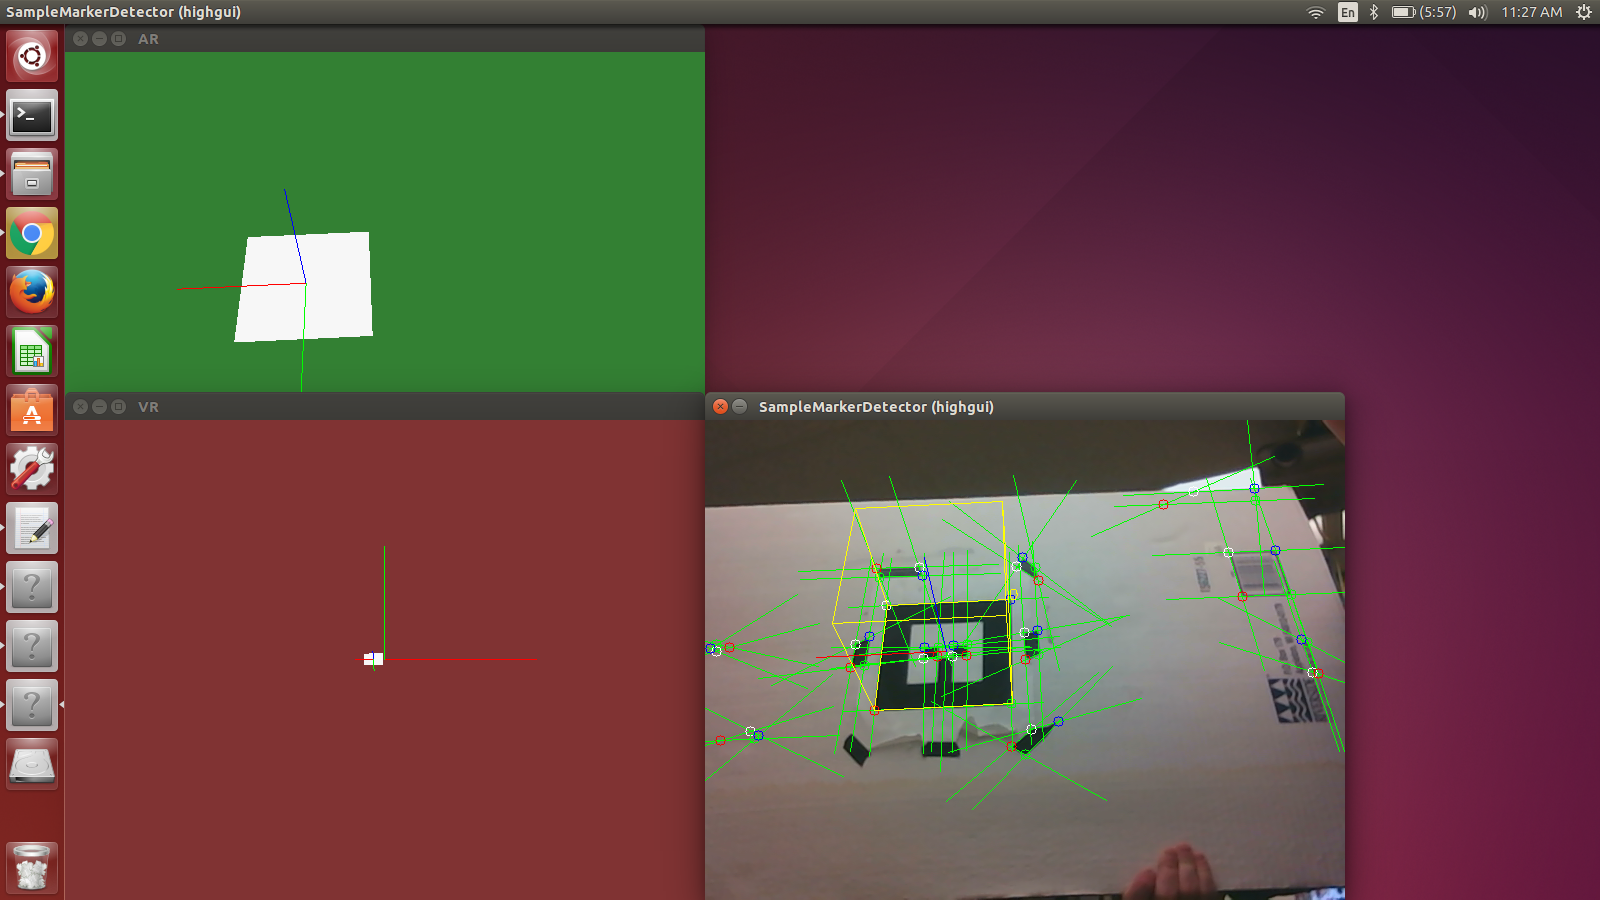
\includegraphics[width=8cm]{AlvarExample.png}
\centering
\caption{ALVAR AR Tracker testing with laptop webcam}
\label{fig:artracker}
\end{figure}

\end{itemize}


\vspace{3mm}
\noindent \large{\textbf{As an owner, I want the UAV to autonomously land on the landing pad with the correct orientation.}}
\normalsize
\begin{itemize}
\item \textbf{Landing Algorithm Simulation}\\
As mentioned previously, as our simulation development has ended, our team will utilize the sensors to generate log data to evaluate. The team will specifically test for orientation corrections that will provide the correct alignment on landing.
\item \textbf{Modify/Rewrite implementation as necessary}\\
As mentioned previously, our visual landing approach has changed. We hope to be able to easily modify the existing software to provide information regarding the orientation of the AR tag to use to change the orientation of the UAV as necessary during landing.
\end{itemize}

\vspace{6mm}
\noindent\Large{\textbf{Prototype}}\\
\normalsize
Our prototype for this sprint is mainly just an assembled hexrotor UAV that is able to follow GPS waypoints. Throughout the assembly process, we did small tests to be sure that we were on the right track. At first, we just kept the UAV in the lab and turned to rotors to verify that they were wired correctly and spinning in the right directions. We then had a manual test flight in the gym, where we discovered that the UAV is quite stable and responsive. Finally, we tested the GPS waypoint navigation with a series of flights. We started small, just having the UAV fly to the end of the driveway at first, eventually working our way up to having the UAV take off, move through a series of waypoints, and return to land on the same location it took off from. Over the course of our testing, we estimate that we will be able to trust the GPS to get us above our landing pad. As stated above, this means that we feel confident that we will be able to trust GPS to get us directly above the landing pad. \newline\newline
We have videos of these GPS tests up on \href{https://www.youtube.com/channel/UCfcuqDXKMLgbUWu3rt9rITA}{YouTube}.




\end{document}